\documentclass[11pt,a4paper]{scrartcl}
\usepackage[utf8]{inputenc}
\usepackage[T1]{fontenc}
\usepackage[ngerman]{babel}
\usepackage{geometry}
\usepackage{graphicx}
\usepackage{hyperref}
\usepackage{caption}
\usepackage{float}
\usepackage{minted}
\usepackage{parskip}

\begin{document}

\section{UART TX}

\begin{figure}[!htbp]
  \centering
  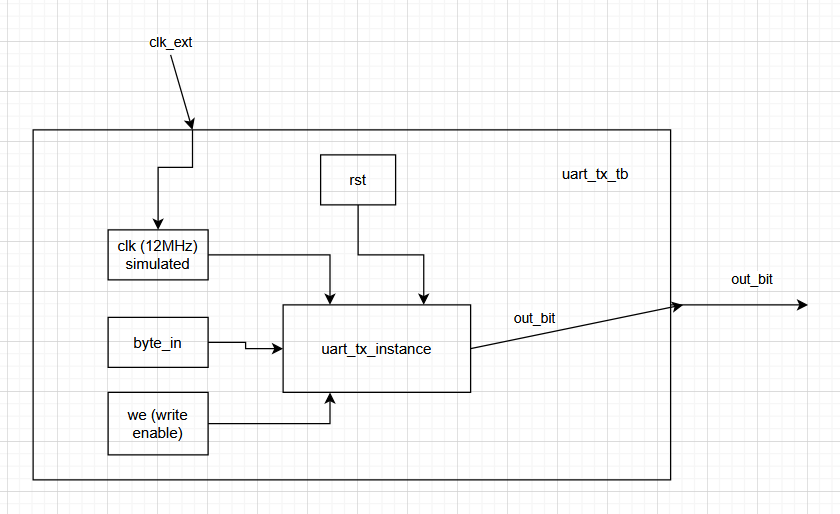
\includegraphics[width=\textwidth]{res/A4_tx_blockdiagram.png}
  \caption{UART TX Blockdiagramm}
\label{fig:uart_tx blockdiagram}  
\end{figure}

Das obige Blockdiagramm zeigt die Struktur des UART TX Moduls. Es besteht aus einem 
Hauptmodul \texttt{uart\_tx} und einem Testbench-Modul \texttt{uart\_tx\_tb}. 
Das Hauptmodul implementiert die UART TX Funktionalität, während das Testbench-Modul zur Simulation und Verifikation der Funktionalität des Hauptmoduls dient.
Der clk-extern Eingang zeigt den tatsächlichen Clock-Eingang, falls eine externe Clock verwendet werden würde. Da wir jedoch die simulierte Clock
der Testbench verwenden, ist dieser Eingang nur symbolisch. 
Die Signale rst, clk \(12MHz\), byte\_in und we werden von der Testbench erzeugt, um die Funktionalität des UART TX Moduls zu testen.

\newpage

\begin{figure}[!htbp]
  \centering
  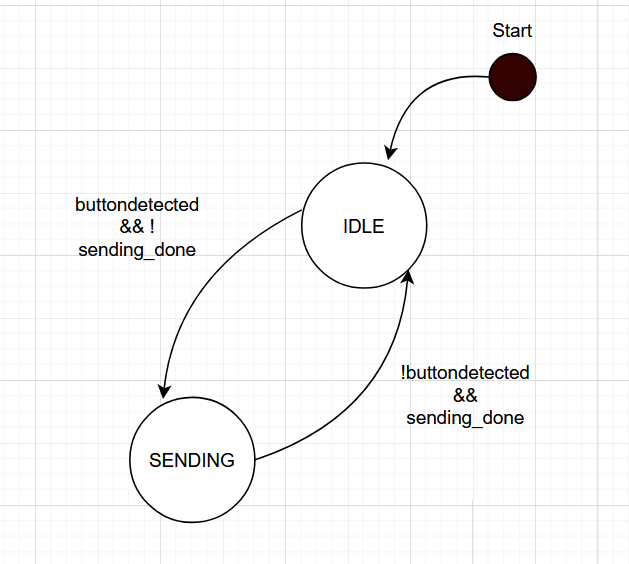
\includegraphics[width=\textwidth]{res/A4_tx_statemaschine.png}
  \caption{UART TX Statusmaschine}
\label{fig:uart_tx statemaschine}  
\end{figure}

Die Statemaschine des UART TX Moduls besteht aus zwei Hauptzuständen: \texttt{IDLE} und \texttt{SENDING}. Der Automat ist deterministisch.

\newpage

\begin{minted}[linenos,breaklines,fontsize=\small]{vhdl}
library ieee;
use IEEE.std_logic_1164.all;
use IEEE.numeric_std.all;

entity uart_tx is
        port(
            clk : in std_logic;
            byte_in : in std_logic_vector(7 downto 0);
            we : in std_logic;
            out_bit : out std_logic;
            rst : in std_logic
        );
    end entity;


architecture uart_tx_a of uart_tx is
    type state_type is (IDLE, SENDING);
    signal state : state_type := IDLE;
    signal symbol_cnt : integer := 0;
    constant baud_rate : integer := 9600;
    constant clk_speed : integer := 12000000;
    constant bit_period : integer := clk_speed / baud_rate;
    signal sending_done : std_logic := '0';
    signal button_detected :std_logic := '0';

begin
    process(clk) is
    variable cnt_period : integer := 0;
    variable start_bit_done : std_logic := '0';
    variable char_bits_done : std_logic := '0';
        begin
            if rising_edge(clk) then

                if rst = '1' then
                    state <= IDLE;
                    out_bit <= '1';
                else 

                    if button_detected = '1' then
                        state <= SENDING;
                        button_detected <= '0';
                    elsif sending_done = '1' then
                        state <= IDLE;
                        sending_done <= '0';
                    end if;

                    case state is
                        when IDLE =>
                        if we = '1' then
                            button_detected <= '1';
                        else
                            out_bit <= '1';
                        end if;
                        when SENDING =>
                            if start_bit_done = '0' then
                                out_bit <= '0';
                                if cnt_period < bit_period then
                                    cnt_period := cnt_period + 1;
                                else
                                    cnt_period := 0;
                                    start_bit_done := '1';
                                end if;
                            elsif char_bits_done = '1' then
                                out_bit <= '1';
                                if cnt_period < bit_period then
                                    cnt_period := cnt_period + 1;
                                else
                                    cnt_period := 0;
                                    char_bits_done := '0';
                                    start_bit_done := '0';
                                    sending_done <= '1';
                                end if;
                            else
                                if symbol_cnt < 8 then

                                    out_bit <= byte_in(symbol_cnt);
                                    cnt_period := cnt_period + 1;

                                    if cnt_period > (bit_period - 1 ) then
                                        symbol_cnt <= symbol_cnt + 1;
                                        cnt_period := 0;
                                    end if;
                                else
                                    symbol_cnt <= 0;
                                    char_bits_done := '1';
                                end if;
                            end if;

                                
                    end case;
                
                end if;

            end if;
    end process;
end architecture uart_tx_a;
\end{minted}

Vor dem Case-Statement wird geprüft ob eine der Zustandsübergangskriterien erfüllt ist. Wenn der we-Eingang aktiv ist, wird das 
Zustandsübergangssignal button\_detected auf '1' gesetzt, wodurch der Übergang von IDLE zu SENDING ausgelöst wird.
Sobald das Senden abgeschlossen ist, wird das Zustandsübergangssignal sending\_done auf '1' gesetzt, wodurch der Übergang von SENDING zu IDLE ausgelöst wird.

\newpage

\begin{minted}[linenos,breaklines,fontsize=\small]{vhdl}
library ieee;
use IEEE.std_logic_1164.all;
use IEEE.numeric_std.all;

entity uart_tx_tb is
end entity;


architecture uart_tx_tb_a of uart_tx_tb is
    signal clk : std_logic := '0';
    signal byte_in : std_logic_vector(7 downto 0) := (others => '0');
    signal we : std_logic := '0';
    signal rst : std_logic := '0';
    signal out_bit :std_logic := '0';

begin
        uart_tx_inst : entity work.uart_tx
        port map(
            clk=> clk,
            byte_in => byte_in,
            we => we,
            rst => rst,
            out_bit => out_bit
        );

    clk <= not clk after 83.33 ns / 2;

    process
    begin
        -- Reset
        rst <= '1';
        wait for 100 ns;
        rst <= '0';

        -- Check IDLE
        wait for 50 ns;
        assert out_bit = '1' report "ERROR: out_bit not idle high after reset" severity error;

        -- 1
        byte_in <= "11010001";
        wait for 100 ns;
        we <= '1';
        wait for 100 ns;
        we <= '0';

        wait for 50 us;
        assert out_bit = '0'
            report "ERROR: Startbit not detected (Test 1)"
            severity warning;

        wait for 2 ms;
        assert out_bit = '1'
            report "ERROR: Line not back to idle (Test 1)"
            severity error;

        -- 2
        byte_in <= "10101010";
        wait for 100 ns;
        we <= '1';
        wait for 300 ns;
        we <= '0';

        wait for 50 us;
        assert out_bit = '0'
            report "ERROR: Startbit not detected (Test 2)"
            severity warning;

        wait for 2 ms;

        -- 3
        byte_in <= "11110000";
        wait for 100 ns;
        we <= '1';
        wait for 300 ns;
        we <= '0';

        wait for 50 us;
        assert out_bit = '0'
            report "ERROR: Startbit not detected (Test 3)"
            severity warning;

        wait for 2 ms;

        -- 4
        byte_in <= "00001111";
        wait for 100 ns;
        we <= '1';
        wait for 300 ns;
        we <= '0';

        wait for 50 us;
        assert out_bit = '0'
            report "ERROR: Startbit not detected (Test 4)"
            severity warning;

        wait for 2 ms;

        -- 5
        byte_in <= "00110011";
        wait for 100 ns;
        we <= '1';
        wait for 300 ns;
        we <= '0';

        wait for 50 us;
        assert out_bit = '0'
            report "ERROR: Startbit not detected (Test 5)"
            severity warning;

        wait for 2 ms;

        -- Ende
        assert false report "Simulation finished successfully" severity note;
        wait;


    end process;
end architecture uart_tx_tb_a;
\end{minted}

Die Testbench testet fünf mal die Funktionsalität des TX Moduls. Es werden jeweils verschiedene Byte-Werte gesendet.
 Nach jedem Senden wird überprüft, ob das Startbit korrekt erkannt wurde und ob die Leitung nach dem Senden wieder auf den Idle-Zustand zurückkehrt.
Die Asserts dienen zur Fehlererkennung. Schlägt keines der Asserts fehl, so wird am Ende der Simulation eine Erfolgsmeldung ausgegeben.
Die folgenden drei Bilder zeigen drei der Tests aus der Simulation. 
Zu sehen ist, dass die Variable symbol\_cnt von 0 bis 7 hochzählt und, dabei die entsprechenden Bits des byte\_in-Signals auf das out\_bit-Signal überträgt. 
Auch die Funktionalität der Start- und Stoppbits ist gut zu erkennen.

\begin{figure}[!htbp]
  \centering
  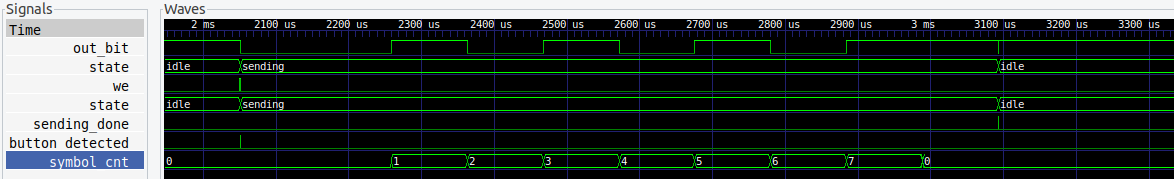
\includegraphics[width=\textwidth]{res/tx_simulation1.png}
  \caption{UART TX Simulation 1}
\label{fig:uart_tx simulation 1}  
\end{figure}

Testcase 2 zeigt die Übertragung des Byte-Werts ''10101010''.

\begin{figure}[!htbp]
  \centering
  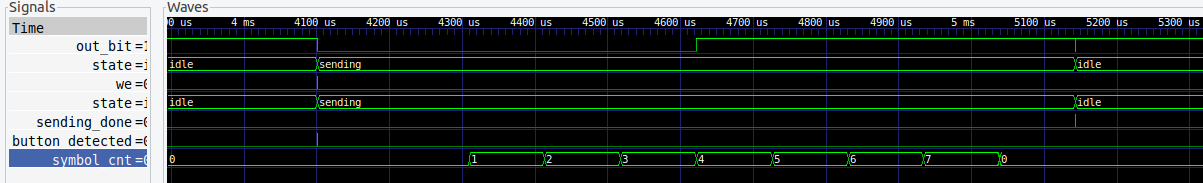
\includegraphics[width=\textwidth]{res/tx_simulation2.png}
  \caption{UART TX Simulation 2}
\label{fig:uart_tx simulation 2}  
\end{figure}

Testcase 3 zeigt die Übertragung des Byte-Werts ''11110000''.

\begin{figure}[!htbp]
  \centering
  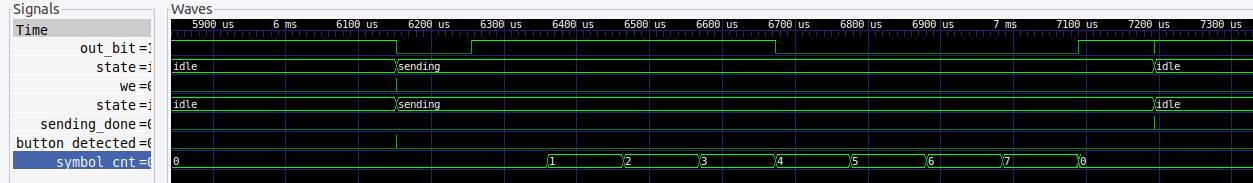
\includegraphics[width=\textwidth]{res/tx_simulation3.png}
  \caption{UART TX Simulation 3}
\label{fig:uart_tx simulation 3}  
\end{figure}

Testcase 4 zeigt die Übertragung des Byte-Werts ''00001111''.

\end{document}
